\documentclass[11pt,titlepage,fleqn]{article}

\usepackage{amsmath}
\usepackage{amssymb}
\usepackage{latexsym}
\usepackage[round]{natbib}
\usepackage{xspace}
\usepackage{graphicx}
\usepackage{epstopdf}
%\usepackage{epsfig}

\usepackage{pifont}   % search for \ding

%\usepackage{fancyhdr}
%\pagestyle{fancy}

%=====================================================
%       SPACING COMMANDS (Latex Companion, p. 52)
%=====================================================

\usepackage{setspace}

%---------------------------
\newcommand{\matlab}{\textsc{Matlab}\xspace}
%---------------------------
\renewcommand{\baselinestretch}{1.0}

\textwidth 460pt
\textheight 700pt
\oddsidemargin 0pt
\evensidemargin 0pt

% see Latex Companion, p. 85
\voffset     -50pt
\topmargin     0pt
\headsep      20pt
\headheight    0pt
\footskip     30pt
\hoffset       0pt

\include{carlcommands}
%\input{dp_header}

\graphicspath{
  {/home/vipul/REPOSITORIES/IITR_seismo/classes/ES510/latex/figures/}
  }

\begin{document}

\noindent Course: Numerical Methods and Computer Programming\\
\noindent Code: ES 510\\
\noindent Instructor: Vipul Silwal (\verb+vsilwalfes@iitr.ac.in+) \\ 
\noindent Last Compiled: \today \\

{\huge Methods for solving ordinary differential equations}

\tableofcontents
%% ------------------------------------------------------------------------ %%
\begin{section}{Difference between ode and pde}
If the equation contains {\it ordinary} derivative of the unknown function $f(x,t)$, \ie $\frac{df}{dt}$, it is an ordinary differential equation. In this case the function will depend on only one independent variable. However, the second 

If the equation contains {\it partial} derivative of the unknown function $f(x,t)$, \ie $\frac{\partial f}{dt}$, and/or, $\frac{\partial f}{dt}$, it is a partial differential equation. Example, wave equation:
\begin{equation}
\frac{\partial ^2 u}{\partial t^2} = c^2 \frac{\partial ^2 u}{\partial x^2}
\end{equation}
where $u(x,t)$ is the displacement at point $x$ at time $t$, with $c$ being the wave propagation speed.

The highest derivative is the {\it order} of the differential equation. The degree of the highest order derivative (remove the square-roots if any).
\end{section}

%-----------------------------------------------------
\begin{section}{Example of an ODE}
{\bf Example 1:}
\begin{eqnarray*}
y' &=& \frac{dy}{dx} = \cos x\\
y &=& \sin x + C
\end{eqnarray*}
where $C$ is the constant. The resulting soluting is a family of solutions (or a general solution). To get a particular solution we will need value of $y$ at some particular $x$; this is called an initial value problem.

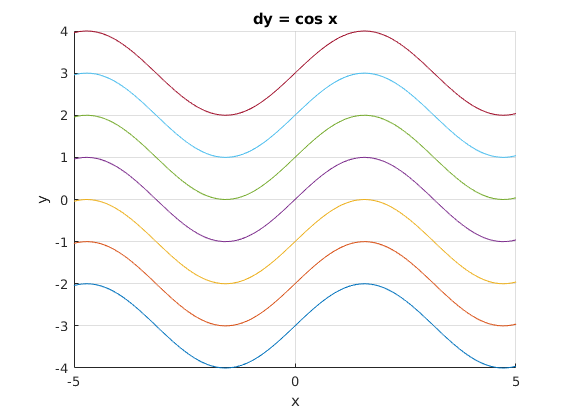
\includegraphics[scale=0.5]{ode_cosx.png}
\end{section}

{\bf Example 2: Exponential growth}
\begin{eqnarray*}
y' &=& \frac{dy}{dx} = 3y\\
\int \frac{dy}{y} &=& 3 \int dx \\
\log(y) + C_1 &=& 3x \\
y &=& e^{3x - C_1} \\
y &=& Ce^{3x}
\end{eqnarray*}
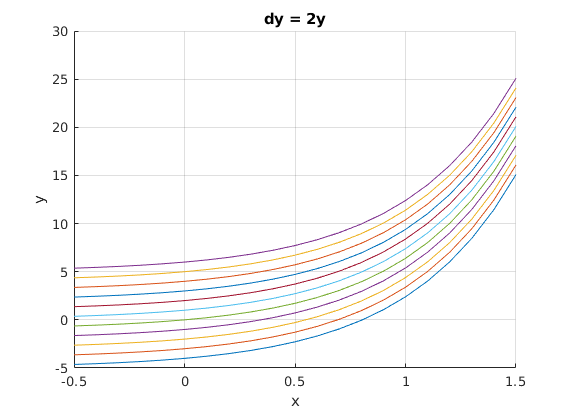
\includegraphics[scale=0.5]{ode_2y.png}

\begin{subsection}{Direction Fields}
Direction fields are used to get an idea about the solution of differential equation without actually having to solve it.

{\bf Example: Newton's second law}

Consider an example of a falling object: mass = 2 kg, air drag = $\gamma = 0.392$.
\begin{eqnarray*}
m \frac{dv}{dt} &=& mg - \gamma v \\
\frac{dv}{dt} &=& g - \frac{\gamma v}{m}\\
\frac{dv}{dt} &=& 9.8 - 0.196 v
\end{eqnarray*}

Now lets plot the family of solutions:

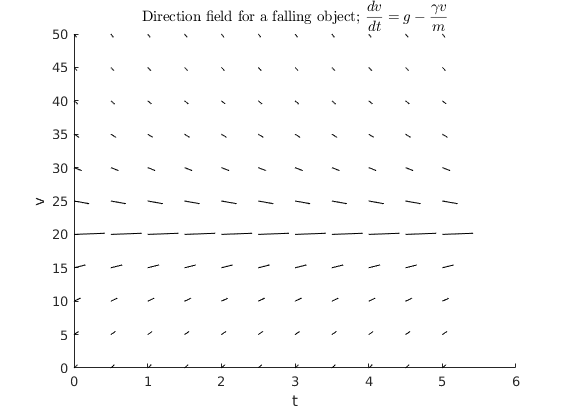
\includegraphics[scale=0.75]{direction_field_falling_object.png}

{\bf Example: $y' = 2 cos(x
) cos(y)$}

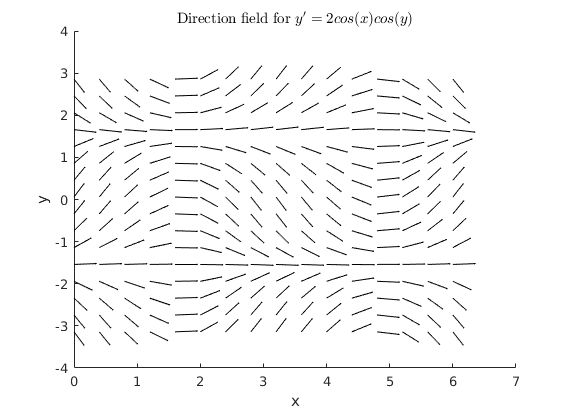
\includegraphics[scale=0.75]{direction_field_2.png}

\end{subsection}
%-----------------------------------------------------

\begin{section}{Euler's Method}
Most of the times differential equation cannot be solved analytically. In such cases numerical approximation can be used to get the unique solutions to the IVP.

\begin{equation}
\frac{dy}{dx} = f(x,y), \hspace{1cm} y(x_0) = y_0   \label{ode}
\end{equation}

Now the equation of the line tangent to $(x_0,y_0)$ would be: $y(x) = y_0 + m(x - x_0)$, where $m$ is the slope. Here we can replace the slope $m$, using equation \ref{ode}:

\begin{equation*}
y(x) = y_0 + f(x_0,y_0)(x - x_0)
\end{equation*}

We are going to perform this iteratively to get the solution:
\begin{eqnarray*}
y_1 &=& y_0 + f(x_0,y_0)(x_1 - x_0) \\
y_2 &=& y_1 + f(x_1,y_1)(x_2 - x_1) \\
&\vdots&\\
y_{n+1} &=& y_n + f(x_n,y_n)(x_{n+1} - x_n)
\end{eqnarray*}
The discretization in $x$ is generally kept constant throughout.

{\bf Example}
\begin{equation*}
\frac{dy}{dx} = -y
\end{equation*}
which could analytically be solved to: $y = C e^{-x}$. Given the initial condition $y(x=0) = 1$, makes $C=1$.

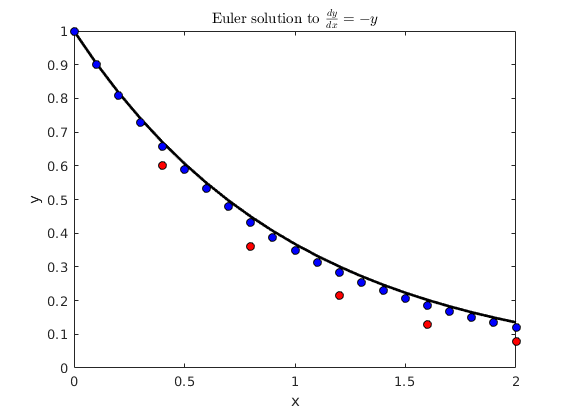
\includegraphics[scale=0.75]{euler.png}


\end{section}
%-----------------------------------------------------

\begin{section}{Runge-Kutta Method}

A wide variety of algorithm comes under this approach. The standard and the classical being the Runga-Kutta fourth-order (RK4) for approximating the solution to the IVP:

\begin{equation}
y' = f(x,y), \hspace{1cm} y(x_0) = y_0
\end{equation}
The solution could be obtained iteratively using:
\begin{equation}
y_{n+1} = y_n + \frac{1}{6} (k_1 + 2k_2 + 2k_3 + k_4)
\end{equation}
where
\begin{eqnarray*}
k_1 &=& h f(x_n,y_n)\\
k_2 &=& h f(x_n + \frac{h}{2},y_n + \frac{k_1}{2})\\
k_3 &=& h f(x_n + \frac{h}{2},y_n + \frac{k_2}{2})\\
k_4 &=& h f(x_{n+1},y_n + k_3)\\
\end{eqnarray*}

\end{section}

\begin{section}{Exercise}
\begin{enumerate}
\item Exponential decay: Solve and plot $ y' = -0.5 y$.

\item Modified Euler's Method (Heun's Method): 

Euler's equation is modified such that the slope used to derive the new $y_{n+1}$ is the average the old slope $f(x_n,y_n)$ and new slope obtained from regular Euler $f(x_{n+1},y_{n+1})$.

\begin{eqnarray*}
y_{n+1}^* &=& y_n + (x_{n+1} - x_n)f(x_n,y_n) \verb+ - origional Euler+\\
y_{n+1} &=& y_n + \frac{(x_{n+1} - x_n)}{2} [f(x_n,y_n) + f(x_{n+1},y_{n+1}^*)] \verb+ - modified Euler+
\end{eqnarray*}

Use this algorithm to solve $y' = y - x$,

Is it same as halving the discretization in x?

\end{enumerate}
\end{section}
\end{document}
